\documentclass{article}
\usepackage{graphicx} % Required for inserting images
\graphicspath{ {Images/} }

\title{CTA200 assignment 3}
\author{Daniel Rogojanski}
\date{May 2023}

\begin{document}

\maketitle

\section*{Question 1}

In this question, I coded the main function called z\_array. This function calls on a function called complex setup which sets up a 100x100 array in which it uses values between -2 and 2 for the x, and complex values in the y direction within the same range. The function then calls the second helper which is called time update, and this function takes a particular index within the 100x100 complex matrix. It iterates it using the questions formula and counts the number of iterations until the value exceeds a predetermined value limit (effectively infinity). To view the output of this question, the view all function outputs the two versions of the data. The left data is coloured by a colour-scale that indicates the iteration number to reach infinity. The right graph displays a di-chromatic display of points that diverge and those who don't diverge. 

\begin{figure}[htp]
    \centering
    \includegraphics[width=12cm]{mandelbrot.pdf}
\end{figure}

\section*{Question 2}

In this question, I first coded up the Lorenz equations in a function aptly named Lorenz. This function is used in later integration steps. I created a function called Lorenz solution which uses some starting parameters and the [$\sigma, r, b$] parameters and calls the Lorenz function with solve ivp to quickly integrate the function. This data was then stored in an array for later use.

To produce figure 1 from Lorenz's paper, I made a function called show figure 1 which takes only the y values and the plots them using matplotlib. I messed around quire a bit with this to try and make it look nice. This output graph seems to be very close to the original as intended. The final output is below. 

\begin{figure}[htp]
    \centering
    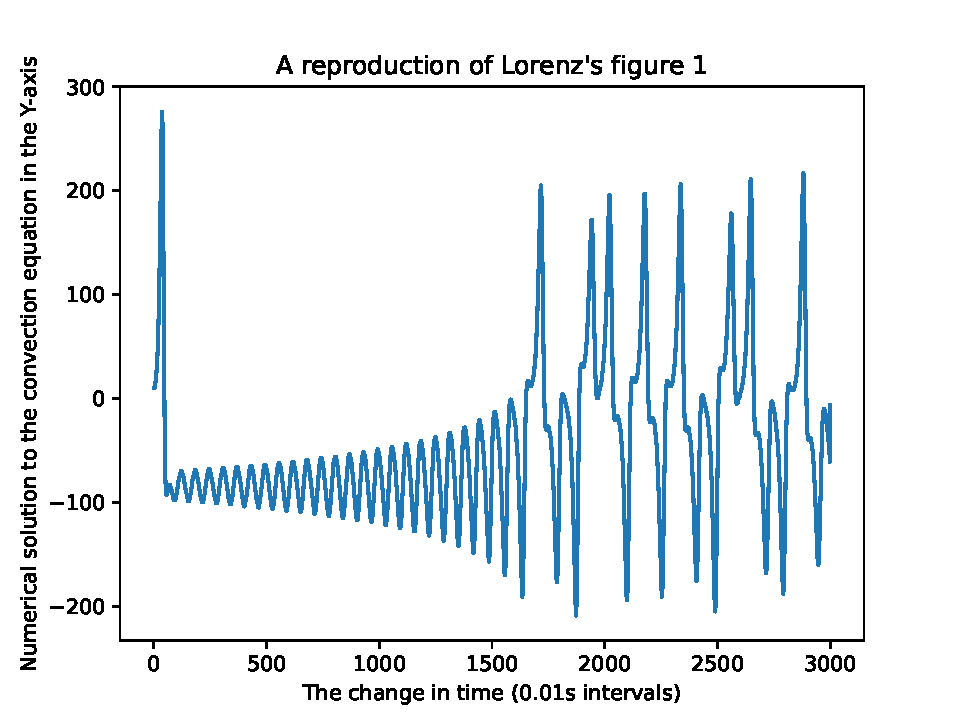
\includegraphics[width=8cm]{Figure_1.pdf}
\end{figure}
          
In order to produce the second figure, I would have to separate the integrated data into its components, and similarly to the first graph, plot x-y and y-z. It took a while to get the graphs to output right, but the output is exactly what would be expected and correlates directly to the second figure in Lorenz's paper. It is shown below.

\begin{figure}[htp]
    \centering
    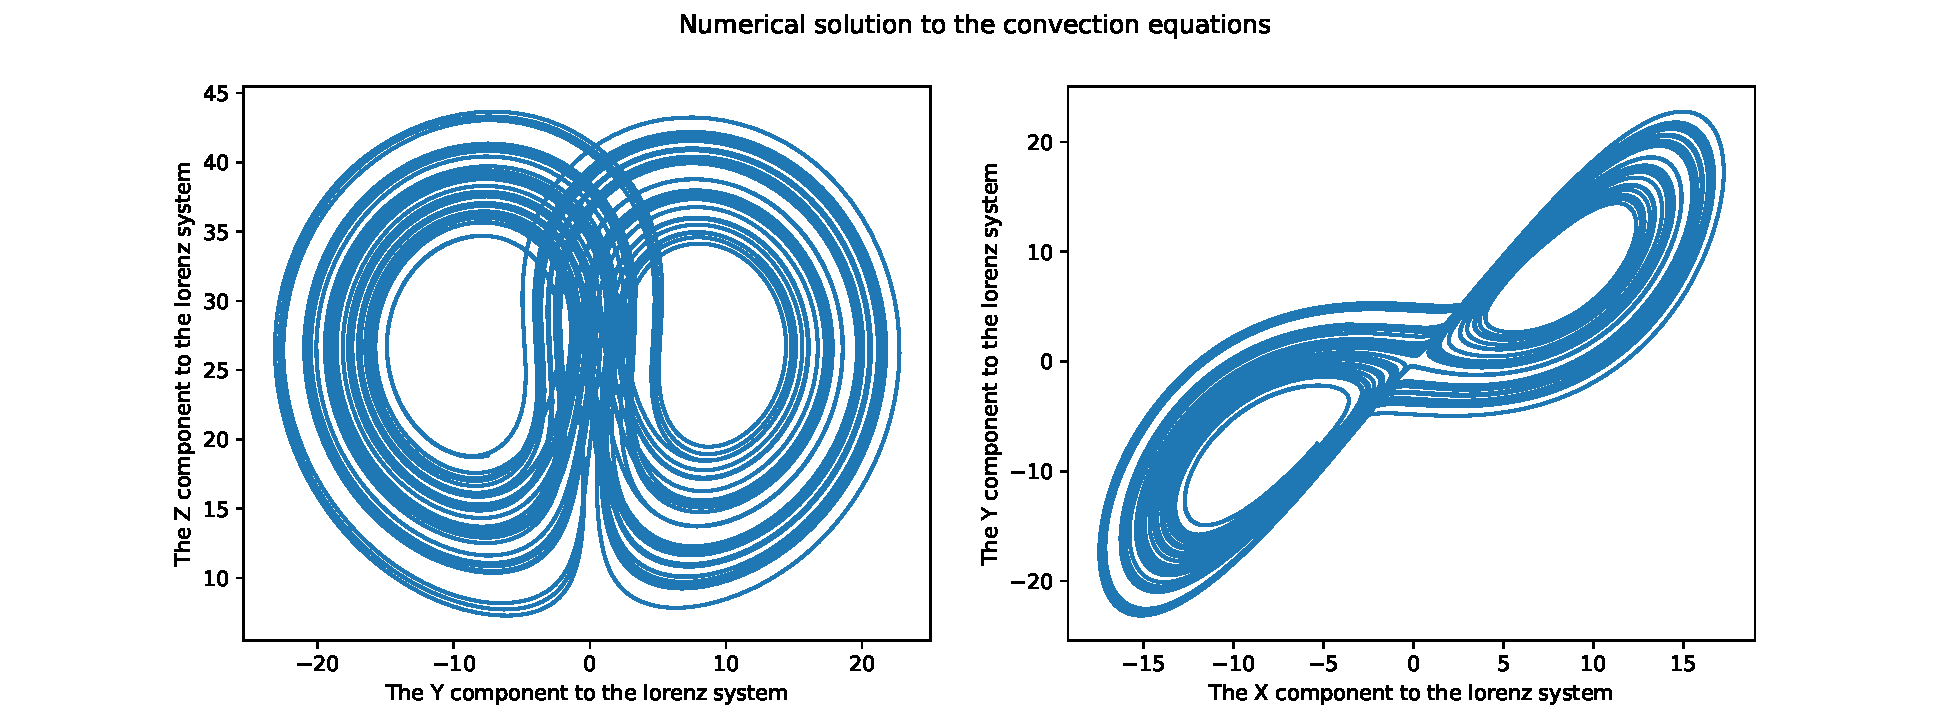
\includegraphics[width=13cm]{Figure_2.pdf}
\end{figure}

Finally, for part 5 of question 2, I went back and made a second copy of the Lorenz solution equation from earlier. In this equation, aptly named slightly different Lorenz, the starting parameters were [0, 1e-8, 0] which made the starting variable very slightly different. I also plotted this function (By just overriding the Lorenz solutions in show figure 2), but did not include it here as it is not required and looks minimally different to the ones already shown. I then took the difference between the coordinates of the original and the slightly modified function, and plotted it using logarithmic scale for the distance and linear scale for the time. This output clearly shown that there is an exponential relation for distance separated over time. It should also be noted that at the top right of the graph, it seems to level out, and this is likely do to the fact that the coordinate points have gotten as separated fro each other as possible given the array constraints. The graph is shown below.

\begin{figure}[htp]
    \centering
    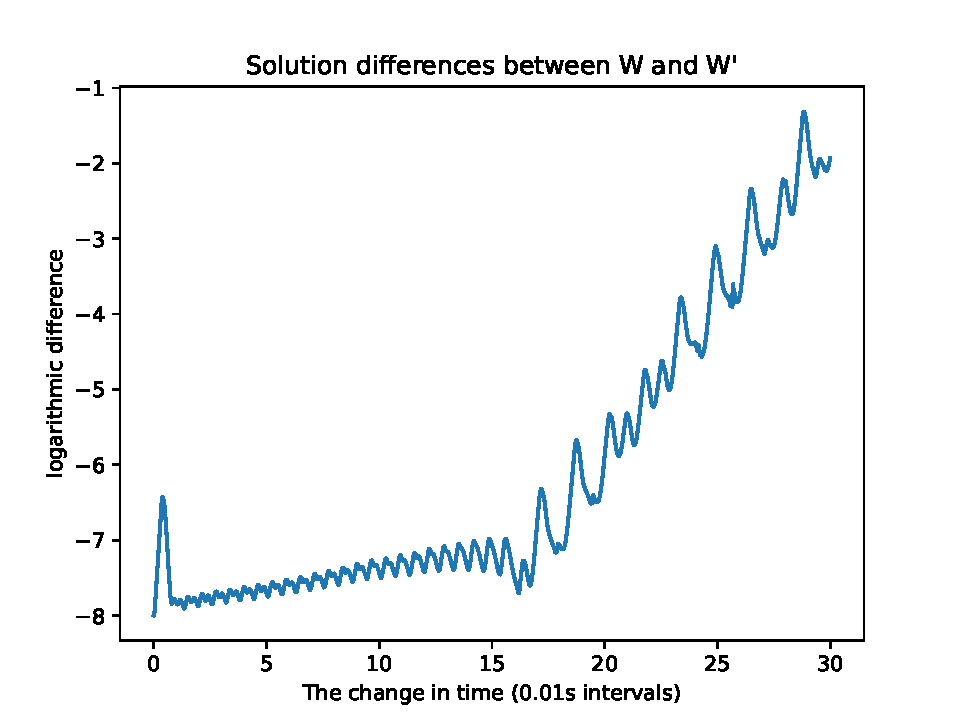
\includegraphics[width=8cm]{Difference_plot.pdf}
\end{figure}

\section*{Question 3}

There is not much to say for this question, I used an online latex editor called overleaf to write all of this and export it. I then uploaded it to my GitHub and that was the end of this assignment. I do not know what else to say here, so goodbye and have a great day!


\end{document}
